%! Author = Anastasia
%! Date = 10.04.2023

% Preamble
\documentclass[a4paper, 12pt, oneside]{scrartcl}
% Packages
\usepackage[T2A]{fontenc}
\usepackage[english, russian]{babel}
\usepackage{amsmath}
\usepackage{graphicx}
\graphicspath{{./Images/}}
\usepackage[utf8]{inputenc}
\usepackage{comment}
\DeclareGraphicsExtensions{.png,.jpg}

\usepackage{listings}
\usepackage{color}
\definecolor{dkgreen}{rgb}{0,0.6,0}
\definecolor{gray}{rgb}{0.5,0.5,0.5}
\definecolor{mauve}{rgb}{0.58,0,0.82}
% Document
\title{Хеширование строк}
\author{}
\date{}
\begin{document}
	\maketitle
	\lstset{frame=tb,
		language=Python,
		aboveskip=3mm,
		belowskip=3mm,
		showstringspaces=false,
		columns=flexible,
		basicstyle={\small\ttfamily},
		numbers=none,
		numberstyle=\tiny\color{gray},
		keywordstyle=\color{blue},
		commentstyle=\color{dkgreen},
		stringstyle=\color{mauve},
		breaklines=true,
		breakatwhitespace=true,
		tabsize=3
	}
	\section{Хеш-функции}\label{sec:section1}
	Хеш-функция предназначена для свертки входного массива любого размера в битовую строку, для MD5 длина выходной строки равна 128 битам. Для чего это нужно?
	К примеру у вас есть два массива, а вам необходимо быстро сравнить их на равенство, то хеш-функция может сделать это за вас, если у двух массивов хеши разные, то массивы гарантировано разные, а в случае равенства хешей — массивы скорее всего равны.
	
	Хеш-функции используются в криптографических алгоритмах, электронных подписях, кодах аутентификации сообщений, обнаружении манипуляций, сканировании отпечатков пальцев, контрольных суммах (проверка целостности сообщений), хеш-таблицах, хранении паролей и многом другом. К примеру, скачивая файл из интернета, вы часто видите рядом с ним строку вида b10a8db164e0754105b7a99be72e3fe5 — это и есть хеш, прогнав этот файл через алгоритм MD5 вы получите такую строку, и, если хэши равны, можно с большой вероятностью утверждать что этот файл действительно подлинный (конечно с некоторыми оговорками, о которых расскажу далее).~\cite{managementsystem}
	
	\section{MD5}\label{sec:section2}
	MD5 (англ. Message Digest 5) — 128-битный алгоритм хеширования, разработанный профессором Рональдом Л. Ривестом из Массачусетского технологического института (Massachusetts Institute of Technology, MIT) в 1991 году.
	Предназначен для создания «отпечатков» или дайджестов сообщения произвольной длины и последующей проверки их подлинности.
	Широко применялся для проверки целостности информации и хранения хешей паролей.
	
	Алгоритм производит хеш со значением в 128 битов. Широко используется для проверки целостности данных.
	Не подходит для использования в иных областях по причине уязвимости в безопасности MD5. (рис.\ref{fig:key})
	\begin{figure}[h!]
		\centering
		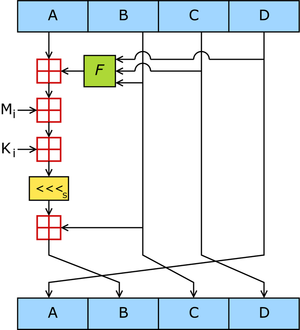
\includegraphics[scale=0.9]{MD5}
		\caption{Схема работы алгоритма MD5}
		\label{fig:key}
	\end{figure}
	\par
	Алгоритм состоит из пяти шагов:\par
	1.Append Padding Bits\par
	В исходную строку дописывают единичный байт 0х80, а затем дописывают нулевые биты, до тех пор, пока длина сообщения не будет сравнима с 448 по модулю 512.
	То есть дописываем нули до тех пор, пока длина нового сообщения не будет равна [длина] = (512*N+448), где N — любое натуральное число, такое, что это выражение будет наиболее близко к длине блока.
	
	2.Append Length\par
	Далее в сообщение дописывается 64-битное представление длины исходного сообщения.
	
	3.Initialize MD Buffer\par
	На этом шаге инициализируется буффер\par
	word A: 01 23 45 67\par
	word B: 89 ab cd ef\par
	word C: fe dc ba 98\par
	word D: 76 54 32 10\par
	Как можно заметить буффер состоит из четырех констант, предназначенный для сбора хэша.\par
	4.Process Message in 16-Word Blocks\par
	На четвертом шаге в первую очередь определяется 4 вспомогательные логические функции, которые преобразуют входные 32-битные слова, в, как ни странно, в 32-битные выходные.\par
	\iffalse
	\begin{equation}
		F(X,Y,Z) = XY v not(X) Z
		\label{Qulon_lo1}
	\end{equation}
	\begin{equation}
		G(X,Y,Z) = XZ v Y not(Z)
		\label{Qulon_lo2}
	\end{equation}
	\begin{equation}
		H(X,Y,Z) = X xor Y xor Z
		\label{Qulon_lo3}
	\end{equation}
	\begin{equation}
		I(X,Y,Z) = Y xor (X v not(Z))
		\label{Qulon_lo4}
	\end{equation}
	\fi
	5.Output\par
	Выводя побайтово буффер ABCD начиная с A и заканчивая D получим наш хеш.\par
	В листинге \ref{some-code} представлен пример MD5-хеширования.\par
	
	\begin{lstlisting}[label=some-code,caption= MD5]
		import hashlib
		hash_object = hashlib.md5(b'Hello World')
		print(hash_object.hexdigest())
	\end{lstlisting}
	\section{SHA-1}\label{sec:section3}
	Default3.
	\bibliography{main}
	\bibliographystyle{plain}
	
\end{document}
